\usetikzlibrary{arrows.meta, positioning}

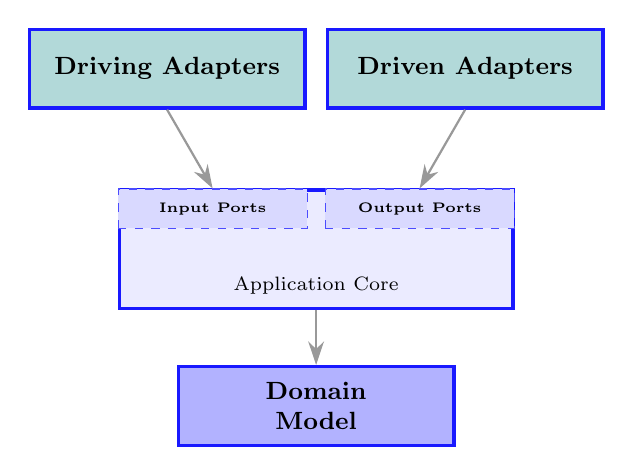
\begin{tikzpicture}[
    node distance=1.5cm and 1cm,
    % Styles
    box/.style={draw=blue!90, fill=blue!8, very thick, align=center, minimum width=3.5cm, minimum height=1.2cm},
    port_box/.style={draw=blue!70, fill=blue!15, dashed, font=\tiny\bfseries, minimum height=0.5cm, minimum width=2.4cm},
    adapter_box/.style={draw=blue!90, fill=teal!30, very thick, align=center, minimum width=3.5cm, minimum height=1cm, font=\small\bfseries},
    domain_box/.style={draw=blue!90, fill=blue!30, very thick, align=center, minimum width=3.5cm, minimum height=1cm, font=\small\bfseries},
    arrow/.style={-{Stealth[length=3mm, width=2mm]}, thick, gray!80}
]

    % 1. APPLICATION CORE
    \node[box, minimum height=1.5cm, minimum width=5cm] (app_core) at (0,0) {};
    % Nudged label slightly lower so it doesn't crowd the ports
    \node[anchor=south, yshift=2pt] at (app_core.south) {\scriptsize Application Core};

    % 2. PORTS
    \node[port_box, anchor=north west] (in_port) at (app_core.north west) {Input Ports};
    \node[port_box, anchor=north east] (out_port) at (app_core.north east) {Output Ports};

    % 3. DOMAIN MODEL - Changed gap from 1.5cm (default) to 0.7cm
    \node[domain_box, below=0.7cm of app_core] (domain) {Domain\\Model};

    % 4. ADAPTERS
    \node[adapter_box, above left=1.0cm and -2.4cm of in_port] (driving) {Driving Adapters};
    \node[adapter_box, above right=1.0cm and -2.4cm of out_port] (driven) {Driven Adapters};

    % 5. ARROWS
    \draw[arrow] (driving.south) -- (in_port.north);
    \draw[arrow] (driven.south) -- (out_port.north);

    % Core to Domain
    \draw[arrow] (app_core.south) -- (domain.north);

\end{tikzpicture}